\section{Introduction}

The Interatomic Coulombic Decay (ICD) is an electronic decay process of an atom or
molecule (a unit) involving atoms or molecules of the environment. After an
ionization from the sub-valence region of a unit $A$, the vacancy is filled
by an electron of the same unit and the excess energy is transferred to a decay
partner $B$, which subsequently get ionized:

\begin{equation*}
 A^+ + B \rightarrow A^+ + B^+ + e^-_{ICD}  .
\end{equation*}

The two units $A$ and $B$ are both positively charged, reppel each other and
thereby undergo a Coulomb explosion. This process was predicted theoretically
\cite{Cederbaum97} and later proven experimentally \cite{Marburger03}. Since then
it has been studied in a multitude of different systems such as small and large
rare gas clusters \cite{many,Fasshauer14_1},
clusters of small molecules \cite{},
quantum dots \cite{Bande13}
and proteins \cite{Harbach13}. Additionally it has given raise to
the investigation of a whole zoo of ICD-like processes (see Ref. \cite{}
and references therein).

The ICD process was so far mostly discussed for the case of decay partners in
the direct vicinity, because the decay widths with decay partners further away
was considered to be negligible. We showed that they need to be included
for larger systems with many decay partners \cite{Fasshauer13} and that the
corresponding peaks are also experimentally observable \cite{Fasshauer14_1}
(see Figure \ref{figure:near_spectra}).
However, this feature has so far not been addressed by itself. We will
therefore first discuss the distance dependency of the ICD in general
in section \ref{} and then
zoom in on the NeNe ICD part of the ICD spectra of NeAr clusters in section
\ref{}. Here we will discuss the peaks and their origin in detail and thereby
raise the question, what a \emph{nearest neighbour} is supposed to be. From
our conclusions we propose the possibility to distinguish cluster structures
of ideal icosahedral and fcc structures using ICD spectra in section \ref{}.

\begin{figure}[h]
 \centering
 \includegraphics[width=\columnwidth]{pics/2dim_coincs.eps}\\
 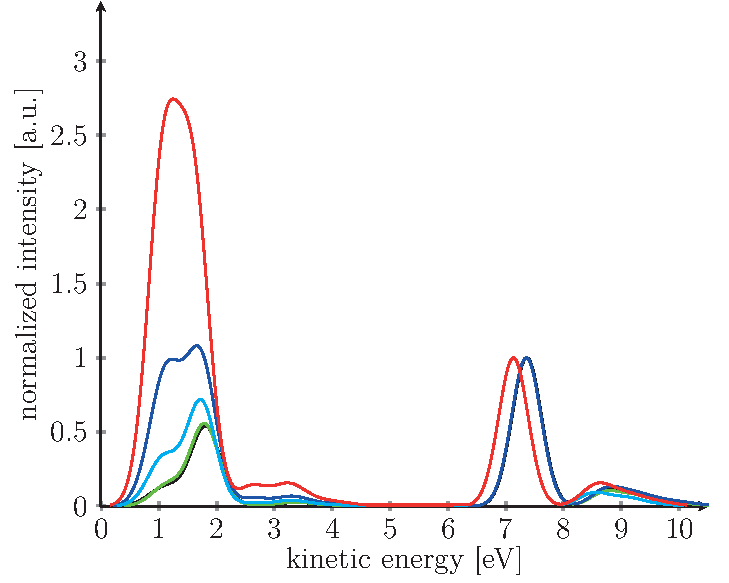
\includegraphics[width=\columnwidth]{pics/NeArcluster_theospecs.pdf}
 \caption{Experimental and theoretical NeAr ICD spectra \cite{Fasshauer14_1}.
          The experimental spectra were obtained for different cluster expansion
          conditions and the theoretical spectra were obtained for different
          underlying cluster structures. In both the NeNe and the NeAr ICD part
          of the spectrum a main peak and next to it at least one more peak at
          higher energies are observed. These smaller peaks stem from decays
          with decay partners at larger distances \cite{Fasshauer13,Fasshauer14_1}.}
 \label{figure:near_spectra}
\end{figure}
